\documentclass[a4paper]{report}

\usepackage[american]{babel}
\usepackage[latin1]{inputenc}
\usepackage{amsmath}
\usepackage{amsfonts}
\usepackage{hyperref}
\usepackage{xspace}
\usepackage{textcomp}
\usepackage{tabularx}
\usepackage{alltt}
\usepackage{url}
\usepackage{vaucanson-g}
\usepackage{graphicx}
\usepackage{tabularx}

\usepackage{listings}
\lstset{%
  numbers=left,
  numberstyle=\tiny,
  stepnumber=5,
  numbersep=5pt,
  firstnumber=1,
  basicstyle=\small,
  frame=single,
  language=C++,
  float}

\newenvironment{cmp}{%
  \begin{center}
    \begin{minipage}{\textwidth}}{%
    \end{minipage}
  \end{center}}

\newcommand{\textrp}[1]{\textit{#1}}
\newcommand{\textarg}[1]{\textsl{#1}}
\newcommand\inputcode[4][]{%
  \begin{figure}[htbp]
    \centering
    \begin{minipage}{0.9\textwidth}
      \lstinputlisting[language=C++, #1]{#2}
    \end{minipage}
    \caption{#3}
    \label{fig:#4}
  \end{figure}}

\usepackage{graphicx}
\graphicspath{{figures/}}

\newcommand{\Vauc}{\textsc{Vaucanson}\xspace}

\title{\Vauc User's manual}
\author{The \Vauc group}
\setcounter{tocdepth}{2}

\makeindex

\begin{document}

\maketitle

\tableofcontents

\chapter{Installation}

\section{Getting \Vauc}

The latest stable version of the \Vauc platform can be downloaded
from \url{http://vaucanson.lrde.epita.fr/}.  The current development
version can be retrieved from its Subversion\footnote{%
%%
  Subversion can be found at \url{http://subversion.tigris.org/}.
%%
} repository as follows:

\begin{shell}
# \kbd{svn checkout https://svn.lrde.epita.fr/svn/vaucanson/trunk vaucanson}
\end{shell}

\section{Building \Vauc}

The following commands build and install the platform (the process
takes an hour on a modern computer):
\begin{shell}
# \kbd{cd vaucanson-1.0}
\end{shell}
Then:
\begin{shell}
# \kbd{./configure}
...
# \kbd{make}
...
# \kbd{sudo make install}
...
\end{shell}

%%% Local Variables:
%%% mode: latex
%%% ispell-local-dictionary: "american"
%%% TeX-master: "vaucanson-user-manual"
%%% End:

\chapter{\Vauc as a toolkit}

\Vauc provides several programs that manipulate various types of
automata. In this chapter we will learn how to use those
programs. Actually there are 6 programs, each of them deals with a
specific type of automata:
\begin{description}
  \item [vcsn-b] for manipulating automata over Boolean semiring $\mathbb{B}$;
  \item [vcsn-z] for manipulating automata over $(\mathbb{Z},+)$;
  \item [vcsn-z\_min\_plus] for manipulating automata over $(\mathbb{Z},min)$;
  \item [vcsn-z\_max\_plus] for manipulating automata over $(\mathbb{Z},max)$;
  \item [vcsn-rt\_tdc] for manipulating realtime transducers;
  \item [vcsn-tdc] for manipulating automata over free monoid product.
\end{description}
The first step before starting to work with \Vauc toolkit is to choose
on which type of automata you intend to work. Then you should just use
the proper program between those listed before.

All automata used in this chapter can be found in the
\textbf{doc/manual/examples/} directory.
\newpage

%%Example on Boolean automaton
\section{Boolean automata}

This part shows the use of the program \textit{b}.

\subsection{A first example}

Let's consider the following Boolean automaton \autoref{A_1}.
%%Schema de l'automate A1
\begin{figure}[ht] \centering
  \begin{VCPicture}{(0,-2)(6,2)}
    % states
    \State{(0,0)}{A} \State{(3,0)}{B} \State{(6,0)}{C}
    % initial--final
    \Initial{A} \Final{C}
    % transitions
    \EdgeL{A}{B}{a} \EdgeL{B}{C}{b}
    \LoopS[.5]{A}{b} \LoopN[.5]{A}{a} \LoopS[.5]{C}{b} \LoopN[.5]{C}{a}
    %
  \end{VCPicture}
  \caption{The automaton $A_1$}
  \label{A_1}
\end{figure}
We will use \Vauc to compute the determinized automaton of $A_1$ and
then we will minimize the resulting automaton.

\subsubsection{Determinization of $A_1$}
Computing the determinized of a Boolean automaton is simply realized
by calling \textit{determinize} function:
\begin{alltt}
# vcsn-b determinize a1.xml > a1\_det.xml
\end{alltt}
Now the file a1\_det.xml contains the XML description of the
determinized of the automaton A.

\subsubsection{Visualizing}

We can get some information about our newly created automaton by calling
the \textit{info} function:
\begin{alltt}
# vcsn-b info a1\_det.xml
\textit{States: 4
Transitions: 8
Initial states: 1
Final states: 2}
\end{alltt}
Or we can use dotty to visualize our newly created automaton:
\begin{alltt}
# vcsn-b display a1\_det.xml
\end{alltt}

%%Dotty output of det(A1)
%%\begin{figure}[ht]
\begin{center}
  \scalebox{0.7}{\includegraphics{images/a1_det.ps}}
\end{center}
%%  \caption{Determinized of $A_1$}
%%\end{figure}

\subsubsection{Minimizing}

The minimal automaton can be computed in the same way:
\begin{alltt}
# vcsn_b minimize a1_det.xml > a1_min.xml
\end{alltt}
The commands can be composed throught the pipe of the shell:
\begin{alltt}
# vcsn_b determinize a1.xml | vcsn_b minimize - > a1_min.xml
\end{alltt}
The '{\tt -}' means that the input is to be read on the standard
input instead of a file.

\subsubsection{Evaluation}

Evaluating if a word is accepted by our automaton:
\begin{alltt}
# vcsn-b eval a1.xml 'abab'
\textit{1}
# vcsn-b eval a1.xml 'bbba'
\textit{0}
\end{alltt}
where 1 (resp. 0) means that the word is accepted (resp. not accepted)
by the automaton.

\subsection{Rational expressions and Boolean automata}

\Vauc provides functions for manipulating rational expressions
associated to Boolean automata. For instance, computing the language
recognized by a Boolean automaton can be done thanks to the
\textit{aut\_to\_exp} function:
\begin{alltt}
# vcsn-b aut-to-exp a1.xml
\textit{(a+b)*.a.b.(a+b)*}
# vcsn-b aut-to-exp a1_det.xml
\textit{b*.a.a*.b.(a.a*.b+b)*.(a.a*+1)}
\end{alltt}
Plus \Vauc provides several algorithms that build an automaton that
recognizes a given language:
\begin{alltt}
# vcsn-b standard "(a+b)*a.b.(a+b)*" | vcsn-b minimize -
\end{alltt}
computes the minimal automaton of $(a+b)*ab(a+b)*$.
%%Please note that your rational expressions should follow the
%%following grammar. %%Fixme : Lien vers la grammaire des ratexp

\subsection{Available functions}
%% Une definition plus rigoureuse des algorithmes devrait etre fournie
%% en annexe.
In this section you will find a brief definition of all functions that
\Vauc provides for manipulating Boolean automata. All these algorithms
are called vcsn-b \textit{algorithm-name} [\textit{arguments}]. If the
argument is replaced by ``-'' then the program will read this argument
from the standard input. All algorithms dump their results to the
standard output, except the ``tests'' functions that also return an
exit status (0 if the test is successfull, anything else otherwise).
In the following:

\begin{itemize}
\item \textarg{a1.xml} and \textarg{a2.xml} are two Boolean automata
  described in \Vauc XML format;
\item \textarg{w} is a word, for example \textit{"aabb"} if you are
  working on an alphabet that contains the letters \textit{a} and
  \textit{b};
\item \textarg{exp} is a rational expression denoting a language;
\item \textarg{n} is a strictly positive integer.
\end{itemize}

\noindent
\begin{tabularx}{\textwidth}{|l|X|}
\hline
\multicolumn{2}{|c|}{Input/output work with automata} \\
\hline
{\tt define-automaton} &Define an automaton from scratch.\\
{\tt edit-automaton} \textarg{a1.xml} & Edit an existing automaton.\\
{\tt info} \textarg{a1.xml} & Print the number of states, transitions,
initial and final states of \textarg{a1.xml}.\\
{\tt display} \textarg{a1.xml} & Display the automaton using DOTTY.\\
{\tt dump} \textarg{a1.xml} & Dump the automaton to DOT format.\\
\hline
\multicolumn{2}{|c|}{Tests and evaluation on automata}\\
\hline
{\tt are-isomorphic} \textarg{a1.xml a2.xml} & Test whether
\textarg{a1.xml} and \textarg{a2.xml} are isomorphic.\\
{\tt evaluation} \textarg{a1.xml w} & Test whether the word
\textarg{w} is accepted by \textarg{a1.xml}.\\
{\tt is-deterministic} \textarg{a1.xml} & Test whether
\textarg{a1.xml} is deterministic.\\
{\tt is-empty} \textarg{a1.xml} & Test whether \textarg{a1.xml}
accepts no word.\\
\hline
\end{tabularx}
\newpage
\begin{tabularx}{\textwidth}{|l|X|}
\hline
\multicolumn{2}{|c|}{Generic algorithms for automata}\\
\hline
{\tt accessible} \textarg{a1.xml} & Extract the sub-automaton of accessible
            states of  \textarg{a1.xml}.\\
{\tt co-accessible} \textarg{a1.xml} & Extract the sub-automaton of
co-accessible states of  \textarg{a1.xml}.\\
{\tt trim} \textarg{a1.xml} & Trim the automaton  \textarg{a1.xml}.\\
{\tt transpose} \textarg{a1.xml} & Compute the automaton accepting the mirror
           language of the one accepted by  \textarg{a1.xml}.\\

{\tt closure} \textarg{[-bf] a1.xml} & $\varepsilon$-removal algorithm.\\
                           & -b : backward closure\\
                           & -f : forward closure\\
{\tt concatenate} \textarg{a1.xml a2.xml} & Concatenate  \textarg{a1.xml}
            to \textarg{a2.xml}.\\
{\tt sum} \textarg{ aut1 aut2} & Compute the sum of  \textarg{a1.xml}
            and \textarg{a2.xml}.\\
{\tt normalize} \textarg{ aut1} & Compute an automaton with unique initial
            and final states, with $\varepsilon$-transitions.\\
{\tt standardize} \textarg{ aut1} & Compute an automaton with unique initial
            state without adding $\varepsilon$-transitions.\\
\hline
\multicolumn{2}{|c|}{Generic algorithms for automata on letters}\\
\hline
{\tt realtime} \textarg{[-bf] a1.xml} & $\varepsilon$-removal
algorithm and make every transition labeled by a letter.\\
                           & -b : backward closure\\
                           & -f : forward closure\\
{\tt product} \textarg{a1.xml a2.xml} & Compute the (cartesian) product
           of  \textarg{a1.xml} and \textarg{a2.xml}.\\
{\tt power} \textarg{a1.xml n} & Compute the (cartesian) product of
\textarg{a1.xml} by itself $n$ times.\\
{\tt quotient} \textarg{a1.xml} & Compute the minimal automaton in
bi-simulation with \textarg{a1.xml}.\\
\hline
\multicolumn{2}{|c|}{Algorithms specific to Boolean automata}\\
\hline
{\tt determinize} \textarg{a1.xml} & Compute the determinized automaton
            of  \textarg{a1.xml}.\\
{\tt complement} \textarg{a1.xml} & Compute an automaton that accepts
the complement language of the one accepted by  \textarg{a1.xml}.\\
{\tt minimize} \textarg{[-hm] a1.xml} & Minimize the {\em deterministic}
           automaton  \textarg{a1.xml}.\\
                           & -h : use the Hopcroft algorithm\\
                           & -m : use the Moore algorithm\\
\hline
\multicolumn{2}{|c|}{Conversion between automata and expressions}\\
\hline
{\tt aut-to-exp} \textarg{a1.xml} & Print a rational expression denoting the
            language accepted by  \textarg{a1.xml}.\\
{\tt expand} \textarg{exp} & Partially expand rational
expressions. For instance, expanding ``a(b+ab(a+b))'' will produce
``aab.(a+b)*+ab''\\
{\tt derived-term} \textarg{exp} & Compute the derived term automaton
           of \textarg{exp}.\\
{\tt standard}  \textarg{exp} & Compute the standard (Glushkov) automaton
           of \textarg{exp}.\\
{\tt thompson-of} \textarg{exp} & Compute the Thompson automaton
           of \textarg{exp}.\\
\hline
\end{tabularx}


\newpage
\section{Transducers}

This section deals with transducers. In \Vauc we distinguish two types
of transducers. The first one is considering a transducer as a
weighted automaton of a product of free monoid (the \textbf{tdc}
program). The second one is considering a transducer as a machine that
takes a word as input and produce another word as output (the
\textbf{rt\_tdc}). One can consider that both views are equivalent and
\Vauc actually provides algorithms to pass from a view to the other one.

\subsection{Example}

The realtime transducer $T_1$(\autoref{bindiv3}) gives the quotient by
3 of a binary number and the transducer $T_2$(\autoref{add1}) adds 1 to a
binary number.


\begin{figure}[h]
  \begin{center}
    \begin{VCPicture}{(0,-2)(6,2)}
% states
\State{(0,0)}{A} \State{(3,0)}{B} \State{(6,0)}{C}
\Initial[w]{A}
\Final[s]{A}
%transitions
\LoopN[.5]{A}{\IOL{0}{0}}
\LoopN[.5]{C}{\IOL{1}{1}}
\ArcL{A}{B}{\IOL{1}{0}}
\ArcL{B}{A}{\IOL{1}{1}}
\ArcL{B}{C}{\IOL{0}{0}}
\ArcL{C}{B}{\IOL{0}{1}}
\end{VCPicture}
\caption{Realtime transducer $T_1$ computing the quotient by 3 of a binary number}
\label{bindiv3}
  \end{center}
\end{figure}
\begin{figure}[h]
  \begin{center}
    \begin{VCPicture}{(0,-2)(3,2)}
% states
\State{(0,0)}{A} \State{(3,0)}{B}
\Initial[w]{A}
\FinalL{s}{A}{(,1)}
\Final[e]{B}
%transitions
\LoopN[.5]{A}{(1,0)}
\LoopN[.5]{B}{(1,1)}
\LoopS[.5]{B}{(0,0)}
\EdgeL{A}{B}{(0,1)}
\end{VCPicture}
\caption{Transducer $T_2$ adding 1 to a binary number}
\label{add1}
  \end{center}
\end{figure}

\subsubsection{Evaluation}
\begin{alltt}
# vcsn-rt_tdc evaluation quot_3_rt.xml '110'
\textit{0.1.0}
\end{alltt}

\subsubsection{Domain}
The transducer $T$ only accepts binary number which are divisible by 3
as input.
\begin{alltt}
# vcsn-rt_tdc domain quot_3_rt.xml > divisible_by_3.xml
\end{alltt}
Now the file divisible\_by\_3.xml contains the description of a Boolean
automaton that accepts only the numbers divisible by 3.

\subsubsection{to-tdc}
Each transucers can be transformed to the other type of transducer
thanks to the ``to-tdc'' and ``to-rt-tdc'' functions.
\begin{alltt}
# vcsn-rt_tdc to-tdc quot_3_rt.xml > quot_3.xml
# vcsn-tdc to-rt-tdc add1.xml > add1_rt.xml
\end{alltt}

\subsubsection{Composing}
\begin{alltt}
# vcsn-tdc compose quot_3.xml add1.xml
\end{alltt}

\subsection{Available functions}
The following functions are available for both vcsn-rt\_tdc and
vcsn-tdc programs. They are called vcsn-\{tdc, rt\_tdc\}
\textit{algorithm-name} [\textit{arguments}].  In the following:

\begin{itemize}
\item \textarg{t1.xml} and \textarg{t2.xml} are two transducers
  (either ``realtime'' or not) described in \Vauc XML format;
\item \textarg{w} is a word, for example \textit{"aabb"} if you are
  working on an alphabet that contains the letters \textit{a} and \textit{b};
\item \textarg{a.xml} is a Boolean automaton;
\item \textarg{t1\_rt.xml} is a realtime transducer;
\item \textarg{t1\_fmp.xml} is a transducer (seen as an automaton over
  a free monoid product).
\end{itemize}

\noindent
\begin{tabularx}{\textwidth}{|l|X|}
\hline
\multicolumn{2}{|c|}{Input/output work with transducers} \\
\hline
{\tt define-automaton} & Define a transducer from scratch.\\
{\tt edit-automaton} \textarg{t1.xml} & Edit an existing transducer.\\
{\tt info} \textarg{t1.xml} & Print the number of states, transitions,
initial and final states of \textit{t1.xml}.\\
{\tt display} \textarg{t1.xml} & Display the transducer using DOTTY.\\


\hline
\multicolumn{2}{|c|}{Tests and evaluation on tranducers}\\
\hline
{\tt are-isomorphic} \textarg{t1.xml t2.xml} & Test if
the two transducers are isomorphic.\\
{\tt evaluation} \textarg{t1.xml w} & Compute the evaluation of
\textit{w} by \textit{t1.xml}.\\
{\tt is-empty} \textarg{t1.xml} & Test if \textit{t1.xml} realizes the
empty relation.\\

\hline
\multicolumn{2}{|c|}{Generic algorithm for tranducers}\\
\hline
{\tt closure} \textarg{t1.xml} & $\varepsilon$-removal algorithm.\\

{\tt compose} \textarg{t1.xml t2.xml} & Compute a tranducer realizing
$f_2 \circ f_1$, where $f_1$ (resp. $f_2$) is the function associated to
\textit{t1.xml} (resp. \textit{t2.xml}).\\

{\tt domain} \textarg{t1.xml} & Compute an automaton accepting all
input accepted by the transducer t1.xml.\\

{\tt evaluation} \textarg{t1.xml} & Compute the evaluation of w by
t1.xml.\\

{\tt evaluation\_aut} \textarg{t1.xml} & Compute a Boolean automaton
describing the words produced by the language described by a.xml
evaluated by t1.xml.\\

{\tt image} \textarg{t1.xml} & Compute an automaton describing all
output produced by the transducer t1.xml.\\

{\tt transpose} \textarg{t1.xml} & Compute the transposed of the
transducer t1.xml.\\


{\tt trim} \textarg{t1.xml} & Compute the trimmed transducer of
t1.xml.\\

\hline
\multicolumn{2}{|c|}{Algorithms for transducers}\\
\hline
{\tt sub-normalize} \textarg{t1\_fmp.xml} & Compute the sub-nomalized
transducer of \textit{t1\_fmp.xml}.\\
{\tt is-sub-normalize} \textarg{t1\_fmp.xml} & Test if
\textit{t1\_fmp.xml} is sub-normalized.\\
{\tt composition-cover} \textarg{t1\_fmp.xml} & .\\%%FIXME
{\tt composition-co-cover} \textarg{t1\_fmp.xml} & .\\%%FIXME
{\tt b-compose} \textarg{t1\_fmp.xml t2\_fmp.xml} & Compose
\textarg{t1\_fmp.xml} and  \textarg{t2\_fmp.xml}. The latters must be
unweighted normalized or sub-normalized transducers.\\
{\tt to-rt-tdc} \textarg{t1\_fmp.xml} & Compute the equivalent
realtime transducer of \textit{t1\_fmp.xml}.\\
{\tt intersection} \textarg{a.xml} & Transform \textarg{a.xml} in a
fmp transducer by creating, for each word, a pair containing twice
this word.\\
\hline
\end{tabularx}
\newpage

\noindent
\begin{tabularx}{\textwidth}{|l|X|}
\hline
\multicolumn{2}{|c|}{Algorithms for ``realtime'' transducers}\\
\hline
{\tt realtime} \textarg{t1\_rt.xml} & Compute the realtime transducer
of  \textit{t1\_rt.xml}.\\
{\tt is-realtime} \textarg(t1\_rt.xml) & Test if \textit{t1\_rt.xml}
is realtime.\\
{\tt to-tdc} \textarg{t1\_rt.xml} & Compute the equivalent fmp
transducer of \textit{t1\_rt.xml}.\\
\hline
\end{tabularx}
\newpage

\section{Weighted automata}

This part shows the use of the program \textit{vcsn-z}, but all
comments should also stand for the programs \textit{vcsn-z\_min\_plus and
vcsn-z\_max\_plus}.

\subsection{Example}

Let's consider the following $\mathbb{N}$-automaton, \textit{i.e.}
an automaton which label's weights are in $\mathbb{N}$:

%%Schema de l'automate B1
\begin{figure}[ht] \centering
  \begin{VCPicture}{(0,-2)(3,2)}
    % states
    \State{(0,0)}{A} \State{(3,0)}{B}
    % initial--final
    \Initial{A} \Final{B}
    % transitions
    \EdgeL{A}{B}{b}
    \LoopS[.5]{A}{b} \LoopN[.5]{A}{a}
    \LoopS[.5]{B}{b} \LoopN[.5]{B}{a}
    %
  \end{VCPicture}
  \caption{The automaton $B_1$}
\end{figure}

This time the evaluation of the word \textit{w} by the automaton $B_1$
will produce a number, rather than simply accept or reject \textit{w}.
For instance let's evaluate "abab" and "bbab":

\subsubsection{Evaluation}

\begin{alltt}
# vcsn-z eval b1.xml 'abbb'
\textit{3}
# vcsn-z eval b1.xml 'abab'
\textit{2}
\end{alltt}

As you may have already guessed the automaton $B_1$ "counts" the
number of 'b' contained in \textit{w}.

\subsubsection{Power}

Now let's consider the $B_1^n$, where
$$B_1^n = \prod_{i=1}^n B_1, n > 0$$

\begin{alltt}
# vcsn-z power b1.xml 4 > b1_4.xml
\end{alltt}

Now the file \textit{b1\_4.xml} contains the automaton $B_1^4$. Lets
see what the evaluation of the words "abab" and "bbab" gives with this
automaton:

\begin{alltt}
# vcsn-z eval b1_4.xml 'bbab'
\textit{81}
# vcsn-z eval b1_4.xml 'abab'
\textit{16}
\end{alltt}

This time one can notice that the automaton $B_1^4$ returns the
evaluation of $B_1$ at power 4.

\subsubsection{quotient}

One drawback of doing successive products of an automaton is
that it creates a lot of new states and transitions.
\begin{alltt}
# vcsn-z power b1.xml 4 | vcsn-z info -
\textit{States: 16}
\textit{Transitions: 97}
\textit{Initial states: 1}
\textit{Final states: 1}
\end{alltt}
One way of reducing the size of our automaton is to use the "quotient"
algorithm.
\begin{alltt}
# vcsn-z power b1.xml 4 | vcsn-z quotient - | vcsn-z info -
\textit{States: 5}
\textit{Transitions: 15}
\textit{Initial states: 1}
\textit{Final states: 1}
\end{alltt}

\subsection{Available functions}
In this section you will find a brief definition of all functions for
manipulating weighted automata. The following functions are available
for both . They are called using vcsn-\{z, z\_max\_plus, z\_min\_plus\}
\textit{algorithm-name} [\textit{arguments}]. In the following:

\begin{itemize}
\item \textarg{a1.xml} and \textarg{a2.xml} are two weighted automata
  described in \Vauc XML format;
\item \textarg{w} is a word, for example \textit{"aabb"} if you are
  working on an alphabet that contains the letters \textit{a} and
  \textit{b};
\item \textarg{exp} is a rational expression denoting a language;
\item \textarg{n} is a strictly positive integer.
\end{itemize}
\newpage

\noindent
\begin{tabularx}{\textwidth}{|l|X|}
\hline
\multicolumn{2}{|c|}{Input/output work with weighted automata}\\
\hline
{\tt define-automaton} & Define an automaton from scratch.\\
{\tt edit-automaton} \textarg{a1.xml} & Edit an existing automaton.\\
{\tt info} \textarg{a1.xml} & Print the number of states, transitions,
initial and final states of \textarg{a1.xml}.\\
{\tt display} \textarg{a1.xml} & Display the automaton using DOTTY.\\


\hline
\multicolumn{2}{|c|}{Tests and evaluation on weighted automata}\\
\hline
{\tt are-isomorphic} \textarg{a1.xml a2.xml} & Test if
the two automata are isomorphic.\\
{\tt evaluation} \textarg{a1.xml w} & Compute the evaluation of
\textarg{w} by \textarg{a1.xml}.\\
{\tt is-empty} \textarg{a1.xml} & .\\
\hline

\hline
\multicolumn{2}{|c|}{Generic algorithms for automata}\\
\hline
{\tt accessible} \textarg{a1.xml} & Extract the sub-automaton of
accessible states of \textarg{a1.xml}.\\
{\tt co-accessible} \textarg{a1.xml} & Extract the sub-automaton of
co-accessible states of \textarg{a1.xml}.\\
{\tt trim} \textarg{a1.xml} & Trim the automaton \textarg{a1.xml}.\\
{\tt transpose} \textarg{a1.xml} & Compute the automaton accepting the
mirror language of the one accepted by \textarg{a1.xml}.\\
{\tt closure} \textarg{[-bf] a1.xml} & $\varepsilon$-removal algorithm.\\
                           & -b : backward closure\\
                           & -f : forward closure\\
{\tt concatenate} \textarg{a1.xml a2.xml} & Concatenate \textarg{a1.xml}
to \textarg{a2.xml}.\\
{\tt sum} \textarg{a1.xml a2.xml} & Compute the sum of \textarg{a1.xml}
and \textarg{a2.xml}.\\
{\tt normalize} \textarg{a1.xml} & Compute an automaton with unique
initial and final states, with $\varepsilon$-transitions.\\
{\tt standardize} \textarg{a1.xml} & Compute an automaton with unique
initial state without adding $\varepsilon$-transitions.\\

\hline
\multicolumn{2}{|c|}{Generic algorithms for automata on letters}\\
\hline
{\tt realtime} \textarg{[-bf] a1.xml} & $\varepsilon$-removal
algorithm and make every transition labeled by a letter.\\
& -b : backward closure\\
& -f : forward closure\\
{\tt product} \textarg{a1.xml a2.xml} & Compute the (cartesian) product
of \textarg{a1.xml} and \textarg{a1.xml}.\\
{\tt power} \textarg{a1.xml n} & Compute the (cartesian) product of
\textarg{a1.xml} by itself $n$ times.\\
{\tt quotient} \textarg{a1.xml} & Compute the $\mathbb{Z}$-quotient of
 \textarg{a1.xml}.\\

\hline
\multicolumn{2}{|c|}{Conversion between automata and expressions}\\
\hline
{\tt aut-to-exp} \textarg{a1.xml} & .\\%%FIXME
{\tt expand} \textarg{exp} & Partially expand rational expressions.\\
{\tt derived-term} \textarg{exp} & Compute the derived term automaton
of \textarg{exp}.\\
{\tt standard}  \textarg{exp} & Compute the standard (Glushkov)
automaton of \textarg{exp}.\\
{\tt thompson-of} \textarg{exp} & Compute the Thompson automaton
of \textarg{exp}.\\
\hline

\end{tabularx}
\newpage

\section{Building your own automaton}
%%FIXME: Here we should give the usage of define_automaton function.

\chapter{\Vauc as a library}


\end{document}